\documentclass[twoside]{book}

% Packages required by doxygen
\usepackage{fixltx2e}
\usepackage{calc}
\usepackage{doxygen}
\usepackage[export]{adjustbox} % also loads graphicx
\usepackage{graphicx}
\usepackage[utf8]{inputenc}
\usepackage{makeidx}
\usepackage{multicol}
\usepackage{multirow}
\PassOptionsToPackage{warn}{textcomp}
\usepackage{textcomp}
\usepackage[nointegrals]{wasysym}
\usepackage[table]{xcolor}

% Font selection
\usepackage[T1]{fontenc}
\usepackage[scaled=.90]{helvet}
\usepackage{courier}
\usepackage{amssymb}
\usepackage{sectsty}
\renewcommand{\familydefault}{\sfdefault}
\allsectionsfont{%
  \fontseries{bc}\selectfont%
  \color{darkgray}%
}
\renewcommand{\DoxyLabelFont}{%
  \fontseries{bc}\selectfont%
  \color{darkgray}%
}
\newcommand{\+}{\discretionary{\mbox{\scriptsize$\hookleftarrow$}}{}{}}

% Page & text layout
\usepackage{geometry}
\geometry{%
  a4paper,%
  top=2.5cm,%
  bottom=2.5cm,%
  left=2.5cm,%
  right=2.5cm%
}
\tolerance=750
\hfuzz=15pt
\hbadness=750
\setlength{\emergencystretch}{15pt}
\setlength{\parindent}{0cm}
\setlength{\parskip}{3ex plus 2ex minus 2ex}
\makeatletter
\renewcommand{\paragraph}{%
  \@startsection{paragraph}{4}{0ex}{-1.0ex}{1.0ex}{%
    \normalfont\normalsize\bfseries\SS@parafont%
  }%
}
\renewcommand{\subparagraph}{%
  \@startsection{subparagraph}{5}{0ex}{-1.0ex}{1.0ex}{%
    \normalfont\normalsize\bfseries\SS@subparafont%
  }%
}
\makeatother

% Headers & footers
\usepackage{fancyhdr}
\pagestyle{fancyplain}
\fancyhead[LE]{\fancyplain{}{\bfseries\thepage}}
\fancyhead[CE]{\fancyplain{}{}}
\fancyhead[RE]{\fancyplain{}{\bfseries\leftmark}}
\fancyhead[LO]{\fancyplain{}{\bfseries\rightmark}}
\fancyhead[CO]{\fancyplain{}{}}
\fancyhead[RO]{\fancyplain{}{\bfseries\thepage}}
\fancyfoot[LE]{\fancyplain{}{}}
\fancyfoot[CE]{\fancyplain{}{}}
\fancyfoot[RE]{\fancyplain{}{\bfseries\scriptsize Generated by Doxygen }}
\fancyfoot[LO]{\fancyplain{}{\bfseries\scriptsize Generated by Doxygen }}
\fancyfoot[CO]{\fancyplain{}{}}
\fancyfoot[RO]{\fancyplain{}{}}
\renewcommand{\footrulewidth}{0.4pt}
\renewcommand{\chaptermark}[1]{%
  \markboth{#1}{}%
}
\renewcommand{\sectionmark}[1]{%
  \markright{\thesection\ #1}%
}

% Indices & bibliography
\usepackage{natbib}
\usepackage[titles]{tocloft}
\setcounter{tocdepth}{3}
\setcounter{secnumdepth}{5}
\makeindex

% Hyperlinks (required, but should be loaded last)
\usepackage{ifpdf}
\ifpdf
  \usepackage[pdftex,pagebackref=true]{hyperref}
\else
  \usepackage[ps2pdf,pagebackref=true]{hyperref}
\fi
\hypersetup{%
  colorlinks=true,%
  linkcolor=blue,%
  citecolor=blue,%
  unicode%
}

% Custom commands
\newcommand{\clearemptydoublepage}{%
  \newpage{\pagestyle{empty}\cleardoublepage}%
}

\usepackage{caption}
\captionsetup{labelsep=space,justification=centering,font={bf},singlelinecheck=off,skip=4pt,position=top}

%===== C O N T E N T S =====

\begin{document}

% Titlepage & ToC
\hypersetup{pageanchor=false,
             bookmarksnumbered=true,
             pdfencoding=unicode
            }
\pagenumbering{alph}
\begin{titlepage}
\vspace*{7cm}
\begin{center}%
{\Large My Project }\\
\vspace*{1cm}
{\large Generated by Doxygen 1.8.13}\\
\end{center}
\end{titlepage}
\clearemptydoublepage
\pagenumbering{roman}
\tableofcontents
\clearemptydoublepage
\pagenumbering{arabic}
\hypersetup{pageanchor=true}

%--- Begin generated contents ---
\chapter{Class Index}
\section{Class List}
Here are the classes, structs, unions and interfaces with brief descriptions\+:\begin{DoxyCompactList}
\item\contentsline{section}{\hyperlink{struct__postfixT}{\+\_\+postfixT} }{\pageref{struct__postfixT}}{}
\end{DoxyCompactList}

\chapter{File Index}
\section{File List}
Here is a list of all documented files with brief descriptions\+:\begin{DoxyCompactList}
\item\contentsline{section}{\hyperlink{buffer_8c}{buffer.\+c} \\*Struct and function for buffer management }{\pageref{buffer_8c}}{}
\item\contentsline{section}{\hyperlink{buffer_8h}{buffer.\+h} \\*Header file for buffer management }{\pageref{buffer_8h}}{}
\item\contentsline{section}{\hyperlink{calculator_8c}{calculator.\+c} \\*Calculator implementation }{\pageref{calculator_8c}}{}
\item\contentsline{section}{\hyperlink{calculator_8h}{calculator.\+h} \\*Header file for Calculator }{\pageref{calculator_8h}}{}
\item\contentsline{section}{\hyperlink{convert_8c}{convert.\+c} \\*Infix-\/to-\/postfix convertor }{\pageref{convert_8c}}{}
\item\contentsline{section}{\hyperlink{convert_8h}{convert.\+h} \\*Header file for infix to postfix convertor }{\pageref{convert_8h}}{}
\item\contentsline{section}{\hyperlink{main_8c}{main.\+c} \\*Calculator program reads the string of numeric infix expression, converts it postfix expression, calculates the postfix expression and prints out the result }{\pageref{main_8c}}{}
\item\contentsline{section}{\hyperlink{stack_8c}{stack.\+c} \\*Stack implementation for symbols }{\pageref{stack_8c}}{}
\item\contentsline{section}{\hyperlink{stack_8h}{stack.\+h} \\*Header file for stack implementation }{\pageref{stack_8h}}{}
\item\contentsline{section}{\hyperlink{utility_8h}{utility.\+h} \\*Utility macros }{\pageref{utility_8h}}{}
\end{DoxyCompactList}

\chapter{Class Documentation}
\hypertarget{classStack}{}\section{Stack Class Reference}
\label{classStack}\index{Stack@{Stack}}
\subsection*{Public Member Functions}
\begin{DoxyCompactItemize}
\item 
\hyperlink{classStack_aa6e4e33ccce6c9a8df6e5519418bbd45}{Stack} (void)
\begin{DoxyCompactList}\small\item\em Default constructor. \end{DoxyCompactList}\item 
\hyperlink{classStack_a8dc60fa32e08d0b556bf66f52e0b8af8}{Stack} (int size)
\begin{DoxyCompactList}\small\item\em Constructor with stack size. \end{DoxyCompactList}\item 
\hyperlink{classStack_a40bd5dff912f0e5290777c4b46d17809}{$\sim$\+Stack} ()
\begin{DoxyCompactList}\small\item\em Destructor. \end{DoxyCompactList}\item 
void \hyperlink{classStack_a974a67de02f49899ec9b4a53e6f8d157}{push} (\hyperlink{structsymbolT}{symbolT} c)
\begin{DoxyCompactList}\small\item\em Push symbol onto stack. \end{DoxyCompactList}\item 
void \hyperlink{classStack_a220c17d4bafbab660762be294d39c3eb}{pop} (\hyperlink{structsymbolT}{symbolT} $\ast$p)
\begin{DoxyCompactList}\small\item\em Pop symbol from stack. \end{DoxyCompactList}\item 
\hyperlink{structsymbolT}{symbolT} \hyperlink{classStack_a5e190884440b0eed5edf06f31d70244f}{top} (void)
\begin{DoxyCompactList}\small\item\em Peek symbol on stack top. \end{DoxyCompactList}\item 
int \hyperlink{classStack_ae340b80cf90a09d5fd6e14efe73f1166}{empty} (void)
\begin{DoxyCompactList}\small\item\em Check if stack is empty. \end{DoxyCompactList}\item 
int \hyperlink{classStack_a30424a3106b7c53dced7c630e35308d6}{full} (void)
\begin{DoxyCompactList}\small\item\em Check if stack is full. \end{DoxyCompactList}\end{DoxyCompactItemize}


\subsection{Constructor \& Destructor Documentation}
\mbox{\Hypertarget{classStack_aa6e4e33ccce6c9a8df6e5519418bbd45}\label{classStack_aa6e4e33ccce6c9a8df6e5519418bbd45}} 
\index{Stack@{Stack}!Stack@{Stack}}
\index{Stack@{Stack}!Stack@{Stack}}
\subsubsection{\texorpdfstring{Stack()}{Stack()}\hspace{0.1cm}{\footnotesize\ttfamily [1/2]}}
{\footnotesize\ttfamily Stack\+::\+Stack (\begin{DoxyParamCaption}\item[{void}]{ }\end{DoxyParamCaption})}



Default constructor. 

\begin{DoxyReturn}{Returns}
N\+O\+NE
\end{DoxyReturn}

\begin{DoxyParams}{Parameters}
{\em N\+O\+NE} & \\
\hline
\end{DoxyParams}
\mbox{\Hypertarget{classStack_a8dc60fa32e08d0b556bf66f52e0b8af8}\label{classStack_a8dc60fa32e08d0b556bf66f52e0b8af8}} 
\index{Stack@{Stack}!Stack@{Stack}}
\index{Stack@{Stack}!Stack@{Stack}}
\subsubsection{\texorpdfstring{Stack()}{Stack()}\hspace{0.1cm}{\footnotesize\ttfamily [2/2]}}
{\footnotesize\ttfamily Stack\+::\+Stack (\begin{DoxyParamCaption}\item[{int}]{size }\end{DoxyParamCaption})}



Constructor with stack size. 

\begin{DoxyReturn}{Returns}
N\+O\+NE
\end{DoxyReturn}

\begin{DoxyParams}{Parameters}
{\em size} & \+: the size of stack \\
\hline
\end{DoxyParams}
\mbox{\Hypertarget{classStack_a40bd5dff912f0e5290777c4b46d17809}\label{classStack_a40bd5dff912f0e5290777c4b46d17809}} 
\index{Stack@{Stack}!````~Stack@{$\sim$\+Stack}}
\index{````~Stack@{$\sim$\+Stack}!Stack@{Stack}}
\subsubsection{\texorpdfstring{$\sim$\+Stack()}{~Stack()}}
{\footnotesize\ttfamily Stack\+::$\sim$\+Stack (\begin{DoxyParamCaption}\item[{void}]{ }\end{DoxyParamCaption})}



Destructor. 

\begin{DoxyReturn}{Returns}
N\+O\+NE
\end{DoxyReturn}

\begin{DoxyParams}{Parameters}
{\em N\+O\+NE} & \\
\hline
\end{DoxyParams}


\subsection{Member Function Documentation}
\mbox{\Hypertarget{classStack_ae340b80cf90a09d5fd6e14efe73f1166}\label{classStack_ae340b80cf90a09d5fd6e14efe73f1166}} 
\index{Stack@{Stack}!empty@{empty}}
\index{empty@{empty}!Stack@{Stack}}
\subsubsection{\texorpdfstring{empty()}{empty()}}
{\footnotesize\ttfamily int Stack\+::empty (\begin{DoxyParamCaption}\item[{void}]{ }\end{DoxyParamCaption})}



Check if stack is empty. 

\begin{DoxyReturn}{Returns}
1, if stack is empty~\newline
0, otherwise
\end{DoxyReturn}

\begin{DoxyParams}{Parameters}
{\em N\+O\+NE} & \\
\hline
\end{DoxyParams}
\mbox{\Hypertarget{classStack_a30424a3106b7c53dced7c630e35308d6}\label{classStack_a30424a3106b7c53dced7c630e35308d6}} 
\index{Stack@{Stack}!full@{full}}
\index{full@{full}!Stack@{Stack}}
\subsubsection{\texorpdfstring{full()}{full()}}
{\footnotesize\ttfamily int Stack\+::full (\begin{DoxyParamCaption}\item[{void}]{ }\end{DoxyParamCaption})}



Check if stack is full. 

\begin{DoxyReturn}{Returns}
1, if stack is empty~\newline
0, otherwise
\end{DoxyReturn}

\begin{DoxyParams}{Parameters}
{\em N\+O\+NE} & \\
\hline
\end{DoxyParams}
\mbox{\Hypertarget{classStack_a220c17d4bafbab660762be294d39c3eb}\label{classStack_a220c17d4bafbab660762be294d39c3eb}} 
\index{Stack@{Stack}!pop@{pop}}
\index{pop@{pop}!Stack@{Stack}}
\subsubsection{\texorpdfstring{pop()}{pop()}}
{\footnotesize\ttfamily void Stack\+::pop (\begin{DoxyParamCaption}\item[{\hyperlink{structsymbolT}{symbolT} $\ast$}]{p }\end{DoxyParamCaption})}



Pop symbol from stack. 

\begin{DoxyReturn}{Returns}
N\+O\+NE
\end{DoxyReturn}

\begin{DoxyParams}{Parameters}
{\em p} & \+: pointer of symbol to return the symbol on stack top \\
\hline
\end{DoxyParams}
\mbox{\Hypertarget{classStack_a974a67de02f49899ec9b4a53e6f8d157}\label{classStack_a974a67de02f49899ec9b4a53e6f8d157}} 
\index{Stack@{Stack}!push@{push}}
\index{push@{push}!Stack@{Stack}}
\subsubsection{\texorpdfstring{push()}{push()}}
{\footnotesize\ttfamily void Stack\+::push (\begin{DoxyParamCaption}\item[{\hyperlink{structsymbolT}{symbolT}}]{c }\end{DoxyParamCaption})}



Push symbol onto stack. 

\begin{DoxyReturn}{Returns}
N\+O\+NE
\end{DoxyReturn}

\begin{DoxyParams}{Parameters}
{\em c} & \+: symbol to push onto stack \\
\hline
\end{DoxyParams}
\mbox{\Hypertarget{classStack_a5e190884440b0eed5edf06f31d70244f}\label{classStack_a5e190884440b0eed5edf06f31d70244f}} 
\index{Stack@{Stack}!top@{top}}
\index{top@{top}!Stack@{Stack}}
\subsubsection{\texorpdfstring{top()}{top()}}
{\footnotesize\ttfamily \hyperlink{structsymbolT}{symbolT} Stack\+::top (\begin{DoxyParamCaption}\item[{void}]{ }\end{DoxyParamCaption})}



Peek symbol on stack top. 

\begin{DoxyReturn}{Returns}
symbol on stack top
\end{DoxyReturn}

\begin{DoxyParams}{Parameters}
{\em N\+O\+NE} & \\
\hline
\end{DoxyParams}


The documentation for this class was generated from the following files\+:\begin{DoxyCompactItemize}
\item 
\hyperlink{stack_8hpp}{stack.\+hpp}\item 
\hyperlink{stack_8cpp}{stack.\+cpp}\end{DoxyCompactItemize}

\hypertarget{structsymbolT}{}\section{symbolT Struct Reference}
\label{structsymbolT}\index{symbolT@{symbolT}}
\subsection*{Public Attributes}
\begin{DoxyCompactItemize}
\item 
\mbox{\Hypertarget{structsymbolT_a82e3326d83d566391f5f07531b596a56}\label{structsymbolT_a82e3326d83d566391f5f07531b596a56}} 
unsigned char \hyperlink{structsymbolT_a82e3326d83d566391f5f07531b596a56}{type}
\begin{DoxyCompactList}\small\item\em indicator of val (operand or operator) \end{DoxyCompactList}\item 
\mbox{\Hypertarget{structsymbolT_a8bcd4f48b8906ca6bf79d5dc4b2814b7}\label{structsymbolT_a8bcd4f48b8906ca6bf79d5dc4b2814b7}} 
int \hyperlink{structsymbolT_a8bcd4f48b8906ca6bf79d5dc4b2814b7}{val}
\begin{DoxyCompactList}\small\item\em parsed value. can be operand or operator \end{DoxyCompactList}\end{DoxyCompactItemize}


The documentation for this struct was generated from the following file\+:\begin{DoxyCompactItemize}
\item 
\hyperlink{buffer_8h}{buffer.\+h}\end{DoxyCompactItemize}

\chapter{File Documentation}
\hypertarget{buffer_8c}{}\section{buffer.\+c File Reference}
\label{buffer_8c}\index{buffer.\+c@{buffer.\+c}}


Struct and function for buffer management.  


{\ttfamily \#include $<$stdio.\+h$>$}\newline
{\ttfamily \#include $<$stdlib.\+h$>$}\newline
{\ttfamily \#include $<$string.\+h$>$}\newline
{\ttfamily \#include $<$errno.\+h$>$}\newline
{\ttfamily \#include $<$buffer.\+h$>$}\newline
Include dependency graph for buffer.\+c\+:\nopagebreak
\begin{figure}[H]
\begin{center}
\leavevmode
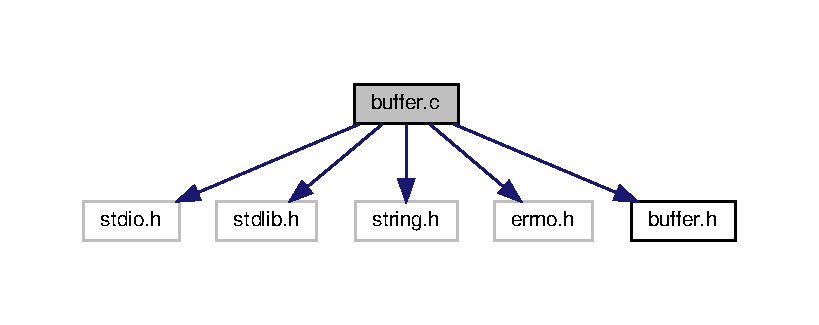
\includegraphics[width=350pt]{buffer_8c__incl}
\end{center}
\end{figure}
\subsection*{Functions}
\begin{DoxyCompactItemize}
\item 
void \hyperlink{buffer_8c_ad750ab66fe8e3301c160ad724023f536}{initialize\+Buffers} (void)
\begin{DoxyCompactList}\small\item\em Initialize infix \& postfix buffers by filling 0x0. \end{DoxyCompactList}\item 
int \hyperlink{buffer_8c_a03b6554bffedbd364eec1ad86bf98d41}{get\+Infix\+Expression} (void)
\begin{DoxyCompactList}\small\item\em Read infix expression via standard input. \end{DoxyCompactList}\item 
char $\ast$ \hyperlink{buffer_8c_ada7435ed756616a3d5b760b5d3886f99}{get\+Infix\+Buffer} (void)
\begin{DoxyCompactList}\small\item\em Return infix buffer. \end{DoxyCompactList}\item 
void \hyperlink{buffer_8c_a618c1585861f39638b6d567ef85c5043}{print\+Infix\+Buffer} (void)
\begin{DoxyCompactList}\small\item\em Print infix buffer. \end{DoxyCompactList}\item 
\hyperlink{structsymbolT}{symbolT} $\ast$ \hyperlink{buffer_8c_a5a51b3f44ff9ca095330fca9f9797eac}{get\+Postfix\+Buffer} (void)
\begin{DoxyCompactList}\small\item\em Return postfix buffer. \end{DoxyCompactList}\item 
void \hyperlink{buffer_8c_afc4e7147ef3990e256a33ec719b7c9e0}{print\+Postfix\+Buffer} (void)
\begin{DoxyCompactList}\small\item\em Print postfix buffer. \end{DoxyCompactList}\item 
void \hyperlink{buffer_8c_a480e702aad3b1bbbda9560444013a473}{print\+Postfix\+Symbol} (\hyperlink{structsymbolT}{symbolT} s)
\end{DoxyCompactItemize}


\subsection{Detailed Description}
Struct and function for buffer management. 

\begin{DoxyDate}{Date}
2018/06/10 
\end{DoxyDate}
\begin{DoxyAuthor}{Author}
Youngeun Park 
\end{DoxyAuthor}


\subsection{Function Documentation}
\mbox{\Hypertarget{buffer_8c_ada7435ed756616a3d5b760b5d3886f99}\label{buffer_8c_ada7435ed756616a3d5b760b5d3886f99}} 
\index{buffer.\+c@{buffer.\+c}!get\+Infix\+Buffer@{get\+Infix\+Buffer}}
\index{get\+Infix\+Buffer@{get\+Infix\+Buffer}!buffer.\+c@{buffer.\+c}}
\subsubsection{\texorpdfstring{get\+Infix\+Buffer()}{getInfixBuffer()}}
{\footnotesize\ttfamily char$\ast$ get\+Infix\+Buffer (\begin{DoxyParamCaption}\item[{void}]{ }\end{DoxyParamCaption})}



Return infix buffer. 

\begin{DoxyReturn}{Returns}
Pointer to infix buffer
\end{DoxyReturn}

\begin{DoxyParams}{Parameters}
{\em N\+O\+NE} & \\
\hline
\end{DoxyParams}
\mbox{\Hypertarget{buffer_8c_a03b6554bffedbd364eec1ad86bf98d41}\label{buffer_8c_a03b6554bffedbd364eec1ad86bf98d41}} 
\index{buffer.\+c@{buffer.\+c}!get\+Infix\+Expression@{get\+Infix\+Expression}}
\index{get\+Infix\+Expression@{get\+Infix\+Expression}!buffer.\+c@{buffer.\+c}}
\subsubsection{\texorpdfstring{get\+Infix\+Expression()}{getInfixExpression()}}
{\footnotesize\ttfamily int get\+Infix\+Expression (\begin{DoxyParamCaption}\item[{void}]{ }\end{DoxyParamCaption})}



Read infix expression via standard input. 

\begin{DoxyReturn}{Returns}
On failure, -\/1 (actually, exits program)~\newline
On encounting comment, 0~\newline
On success, the length of expression ( greater than zero )
\end{DoxyReturn}

\begin{DoxyParams}{Parameters}
{\em N\+O\+NE} & \\
\hline
\end{DoxyParams}
\mbox{\Hypertarget{buffer_8c_a5a51b3f44ff9ca095330fca9f9797eac}\label{buffer_8c_a5a51b3f44ff9ca095330fca9f9797eac}} 
\index{buffer.\+c@{buffer.\+c}!get\+Postfix\+Buffer@{get\+Postfix\+Buffer}}
\index{get\+Postfix\+Buffer@{get\+Postfix\+Buffer}!buffer.\+c@{buffer.\+c}}
\subsubsection{\texorpdfstring{get\+Postfix\+Buffer()}{getPostfixBuffer()}}
{\footnotesize\ttfamily \hyperlink{structsymbolT}{symbolT}$\ast$ get\+Postfix\+Buffer (\begin{DoxyParamCaption}\item[{void}]{ }\end{DoxyParamCaption})}



Return postfix buffer. 

\begin{DoxyReturn}{Returns}
Pointer to postfix buffer
\end{DoxyReturn}

\begin{DoxyParams}{Parameters}
{\em N\+O\+NE} & \\
\hline
\end{DoxyParams}
\mbox{\Hypertarget{buffer_8c_ad750ab66fe8e3301c160ad724023f536}\label{buffer_8c_ad750ab66fe8e3301c160ad724023f536}} 
\index{buffer.\+c@{buffer.\+c}!initialize\+Buffers@{initialize\+Buffers}}
\index{initialize\+Buffers@{initialize\+Buffers}!buffer.\+c@{buffer.\+c}}
\subsubsection{\texorpdfstring{initialize\+Buffers()}{initializeBuffers()}}
{\footnotesize\ttfamily void initialize\+Buffers (\begin{DoxyParamCaption}\item[{void}]{ }\end{DoxyParamCaption})}



Initialize infix \& postfix buffers by filling 0x0. 

\begin{DoxyReturn}{Returns}
N\+O\+NE 
\end{DoxyReturn}
\mbox{\Hypertarget{buffer_8c_a618c1585861f39638b6d567ef85c5043}\label{buffer_8c_a618c1585861f39638b6d567ef85c5043}} 
\index{buffer.\+c@{buffer.\+c}!print\+Infix\+Buffer@{print\+Infix\+Buffer}}
\index{print\+Infix\+Buffer@{print\+Infix\+Buffer}!buffer.\+c@{buffer.\+c}}
\subsubsection{\texorpdfstring{print\+Infix\+Buffer()}{printInfixBuffer()}}
{\footnotesize\ttfamily void print\+Infix\+Buffer (\begin{DoxyParamCaption}\item[{void}]{ }\end{DoxyParamCaption})}



Print infix buffer. 

\begin{DoxyReturn}{Returns}
N\+O\+NE
\end{DoxyReturn}

\begin{DoxyParams}{Parameters}
{\em N\+O\+NE} & \\
\hline
\end{DoxyParams}
\mbox{\Hypertarget{buffer_8c_afc4e7147ef3990e256a33ec719b7c9e0}\label{buffer_8c_afc4e7147ef3990e256a33ec719b7c9e0}} 
\index{buffer.\+c@{buffer.\+c}!print\+Postfix\+Buffer@{print\+Postfix\+Buffer}}
\index{print\+Postfix\+Buffer@{print\+Postfix\+Buffer}!buffer.\+c@{buffer.\+c}}
\subsubsection{\texorpdfstring{print\+Postfix\+Buffer()}{printPostfixBuffer()}}
{\footnotesize\ttfamily void print\+Postfix\+Buffer (\begin{DoxyParamCaption}\item[{void}]{ }\end{DoxyParamCaption})}



Print postfix buffer. 

\begin{DoxyReturn}{Returns}
N\+O\+NE
\end{DoxyReturn}

\begin{DoxyParams}{Parameters}
{\em N\+O\+NE} & \\
\hline
\end{DoxyParams}
\mbox{\Hypertarget{buffer_8c_a480e702aad3b1bbbda9560444013a473}\label{buffer_8c_a480e702aad3b1bbbda9560444013a473}} 
\index{buffer.\+c@{buffer.\+c}!print\+Postfix\+Symbol@{print\+Postfix\+Symbol}}
\index{print\+Postfix\+Symbol@{print\+Postfix\+Symbol}!buffer.\+c@{buffer.\+c}}
\subsubsection{\texorpdfstring{print\+Postfix\+Symbol()}{printPostfixSymbol()}}
{\footnotesize\ttfamily void print\+Postfix\+Symbol (\begin{DoxyParamCaption}\item[{\hyperlink{structsymbolT}{symbolT}}]{s }\end{DoxyParamCaption})}

\begin{DoxyReturn}{Returns}
N\+O\+NE
\end{DoxyReturn}

\begin{DoxyParams}{Parameters}
{\em s} & \+: symbol to print out \\
\hline
\end{DoxyParams}

\hypertarget{buffer_8h}{}\section{buffer.\+h File Reference}
\label{buffer_8h}\index{buffer.\+h@{buffer.\+h}}


Struct and function for buffer management.  


This graph shows which files directly or indirectly include this file\+:\nopagebreak
\begin{figure}[H]
\begin{center}
\leavevmode
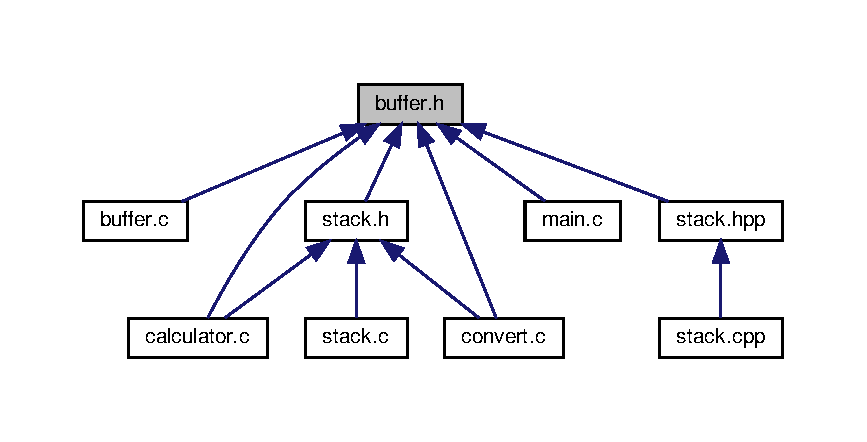
\includegraphics[width=338pt]{buffer_8h__dep__incl}
\end{center}
\end{figure}
\subsection*{Classes}
\begin{DoxyCompactItemize}
\item 
struct \hyperlink{struct__postfixT}{\+\_\+postfixT}
\end{DoxyCompactItemize}
\subsection*{Macros}
\begin{DoxyCompactItemize}
\item 
\mbox{\Hypertarget{buffer_8h_ab5187269936538ffb8ccbbe7115ffdbc}\label{buffer_8h_ab5187269936538ffb8ccbbe7115ffdbc}} 
\#define {\bfseries M\+A\+X\+\_\+\+S\+T\+R\+I\+NG}~1001
\item 
\mbox{\Hypertarget{buffer_8h_a2ea310aceef1f14012a8a85ca3ee7692}\label{buffer_8h_a2ea310aceef1f14012a8a85ca3ee7692}} 
\#define {\bfseries \+\_\+\+N\+O\+N\+E\+\_\+}~0
\item 
\mbox{\Hypertarget{buffer_8h_ab9e2c5e4b20e20e301f106ee346f1a70}\label{buffer_8h_ab9e2c5e4b20e20e301f106ee346f1a70}} 
\#define {\bfseries \+\_\+\+O\+P\+E\+R\+A\+N\+D\+\_\+}~1
\item 
\mbox{\Hypertarget{buffer_8h_a459cf688a83964e55a237262fd9fde1a}\label{buffer_8h_a459cf688a83964e55a237262fd9fde1a}} 
\#define {\bfseries \+\_\+\+O\+P\+E\+R\+A\+T\+O\+R\+\_\+}~2
\item 
\mbox{\Hypertarget{buffer_8h_a49f8deb02dd2c5590ce6e4094fb9c5de}\label{buffer_8h_a49f8deb02dd2c5590ce6e4094fb9c5de}} 
\#define {\bfseries \+\_\+\+P\+A\+R\+E\+N\+T\+H\+E\+S\+I\+S\+\_\+}~3
\item 
\mbox{\Hypertarget{buffer_8h_aa770c0aa5c81cfe98169f0128128e399}\label{buffer_8h_aa770c0aa5c81cfe98169f0128128e399}} 
\#define {\bfseries \+\_\+\+T\+E\+R\+M\+I\+N\+A\+T\+O\+R\+\_\+}~4
\item 
\mbox{\Hypertarget{buffer_8h_a9da9a21c28893857fd6e8436da348c0b}\label{buffer_8h_a9da9a21c28893857fd6e8436da348c0b}} 
\#define {\bfseries Is\+None}(a)~(a.\+\_\+operator == \+\_\+\+N\+O\+N\+E\+\_\+)
\item 
\mbox{\Hypertarget{buffer_8h_a4892cde70001679abd5005eb029a8a8b}\label{buffer_8h_a4892cde70001679abd5005eb029a8a8b}} 
\#define {\bfseries Is\+Operand}(a)~(a.\+\_\+operator == \+\_\+\+O\+P\+E\+R\+A\+N\+D\+\_\+)
\item 
\mbox{\Hypertarget{buffer_8h_a2df20c9f40edb773d65f156744fbcce2}\label{buffer_8h_a2df20c9f40edb773d65f156744fbcce2}} 
\#define {\bfseries Is\+Operator}(a)~(a.\+\_\+operator == \+\_\+\+O\+P\+E\+R\+A\+T\+O\+R\+\_\+)
\item 
\mbox{\Hypertarget{buffer_8h_af7fcc0a4a7bb4b46c50a72406e5bf106}\label{buffer_8h_af7fcc0a4a7bb4b46c50a72406e5bf106}} 
\#define {\bfseries Is\+Parenthesis}(a)~(a.\+\_\+operator == \+\_\+\+P\+A\+R\+E\+N\+T\+H\+E\+S\+I\+S\+\_\+)
\item 
\mbox{\Hypertarget{buffer_8h_a1f600538736a3d312fa826cc3e51cd77}\label{buffer_8h_a1f600538736a3d312fa826cc3e51cd77}} 
\#define {\bfseries Is\+Terminator}(a)~(a.\+\_\+operator == \+\_\+\+T\+E\+R\+M\+I\+N\+A\+T\+O\+R\+\_\+)
\item 
\mbox{\Hypertarget{buffer_8h_ae54365e424e0df26819e85d73c2b34d6}\label{buffer_8h_ae54365e424e0df26819e85d73c2b34d6}} 
\#define {\bfseries S\+I\+Z\+E\+\_\+\+P\+O\+S\+T\+F\+I\+X\+\_\+\+B\+U\+F\+F\+ER}~(sizeof(postfix) / sizeof(\hyperlink{struct__postfixT}{\+\_\+postfixT}))
\end{DoxyCompactItemize}
\subsection*{Functions}
\begin{DoxyCompactItemize}
\item 
void \hyperlink{buffer_8h_a6efdf55f2c7801fd6dfc48baba20ef40}{initialize\+Bufffers} (void)
\begin{DoxyCompactList}\small\item\em Initizize infix \& postfix buffers to fill 0x0. \end{DoxyCompactList}\item 
\mbox{\Hypertarget{buffer_8h_a03b6554bffedbd364eec1ad86bf98d41}\label{buffer_8h_a03b6554bffedbd364eec1ad86bf98d41}} 
int {\bfseries get\+Infix\+Expression} (void)
\item 
\mbox{\Hypertarget{buffer_8h_ada7435ed756616a3d5b760b5d3886f99}\label{buffer_8h_ada7435ed756616a3d5b760b5d3886f99}} 
char $\ast$ {\bfseries get\+Infix\+Buffer} (void)
\item 
\mbox{\Hypertarget{buffer_8h_a618c1585861f39638b6d567ef85c5043}\label{buffer_8h_a618c1585861f39638b6d567ef85c5043}} 
void {\bfseries print\+Infix\+Buffer} (void)
\item 
\mbox{\Hypertarget{buffer_8h_ac8f8d9fa237944a62302a8b3b05b804e}\label{buffer_8h_ac8f8d9fa237944a62302a8b3b05b804e}} 
\hyperlink{struct__postfixT}{\+\_\+postfixT} $\ast$ {\bfseries get\+Postfix\+Buffer} (void)
\item 
\mbox{\Hypertarget{buffer_8h_afc4e7147ef3990e256a33ec719b7c9e0}\label{buffer_8h_afc4e7147ef3990e256a33ec719b7c9e0}} 
void {\bfseries print\+Postfix\+Buffer} (void)
\item 
\mbox{\Hypertarget{buffer_8h_a619156ec223c21bb6ba588113b6febd3}\label{buffer_8h_a619156ec223c21bb6ba588113b6febd3}} 
void {\bfseries print\+Postfix\+Symbol} (\hyperlink{struct__postfixT}{\+\_\+postfixT} s)
\end{DoxyCompactItemize}


\subsection{Detailed Description}
Struct and function for buffer management. 

\begin{DoxyDate}{Date}
2018/06/10 
\end{DoxyDate}
\begin{DoxyAuthor}{Author}
Youngeun Park 
\end{DoxyAuthor}


\subsection{Function Documentation}
\mbox{\Hypertarget{buffer_8h_a6efdf55f2c7801fd6dfc48baba20ef40}\label{buffer_8h_a6efdf55f2c7801fd6dfc48baba20ef40}} 
\index{buffer.\+h@{buffer.\+h}!initialize\+Bufffers@{initialize\+Bufffers}}
\index{initialize\+Bufffers@{initialize\+Bufffers}!buffer.\+h@{buffer.\+h}}
\subsubsection{\texorpdfstring{initialize\+Bufffers()}{initializeBufffers()}}
{\footnotesize\ttfamily void initialize\+Bufffers (\begin{DoxyParamCaption}\item[{void}]{ }\end{DoxyParamCaption})}



Initizize infix \& postfix buffers to fill 0x0. 

\begin{DoxyReturn}{Returns}
N\+O\+NE  N\+O\+NE 
\end{DoxyReturn}

\hypertarget{calculator_8c}{}\section{calculator.\+c File Reference}
\label{calculator_8c}\index{calculator.\+c@{calculator.\+c}}


Calculator implementation.  


{\ttfamily \#include $<$stdio.\+h$>$}\newline
{\ttfamily \#include $<$stdlib.\+h$>$}\newline
{\ttfamily \#include $<$string.\+h$>$}\newline
{\ttfamily \#include $<$buffer.\+h$>$}\newline
{\ttfamily \#include $<$stack.\+h$>$}\newline
{\ttfamily \#include $<$utility.\+h$>$}\newline
Include dependency graph for calculator.\+c\+:\nopagebreak
\begin{figure}[H]
\begin{center}
\leavevmode
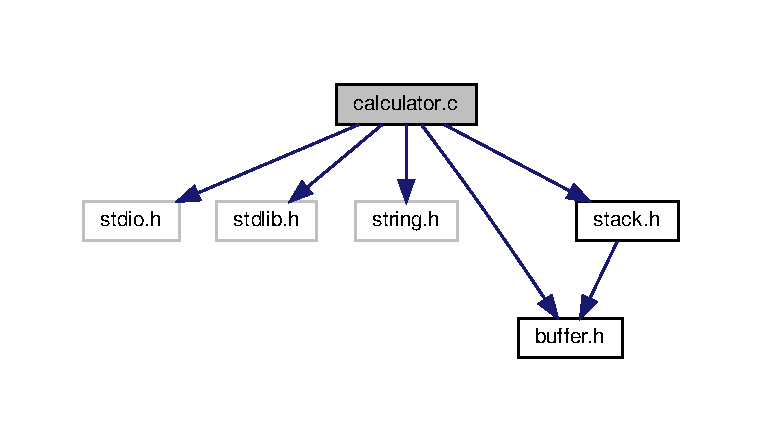
\includegraphics[width=350pt]{calculator_8c__incl}
\end{center}
\end{figure}
\subsection*{Functions}
\begin{DoxyCompactItemize}
\item 
int \hyperlink{calculator_8c_a267908546719af12ada386fa341bfaf8}{calc} (int $\ast$result)
\begin{DoxyCompactList}\small\item\em calculator function to evaluate postifx expression \end{DoxyCompactList}\end{DoxyCompactItemize}


\subsection{Detailed Description}
Calculator implementation. 

\begin{DoxyDate}{Date}
2018/06/10 
\end{DoxyDate}
\begin{DoxyAuthor}{Author}
Youngeun Park 
\end{DoxyAuthor}


\subsection{Function Documentation}
\mbox{\Hypertarget{calculator_8c_a267908546719af12ada386fa341bfaf8}\label{calculator_8c_a267908546719af12ada386fa341bfaf8}} 
\index{calculator.\+c@{calculator.\+c}!calc@{calc}}
\index{calc@{calc}!calculator.\+c@{calculator.\+c}}
\subsubsection{\texorpdfstring{calc()}{calc()}}
{\footnotesize\ttfamily int calc (\begin{DoxyParamCaption}\item[{int $\ast$}]{result }\end{DoxyParamCaption})}



calculator function to evaluate postifx expression 

\begin{DoxyReturn}{Returns}
On success, 1~\newline
On failure, 0
\end{DoxyReturn}

\begin{DoxyParams}{Parameters}
{\em result} & (O\+UT) \+: integer pointer to return calculated result \\
\hline
\end{DoxyParams}

\hypertarget{calculator_8h}{}\section{calculator.\+h File Reference}
\label{calculator_8h}\index{calculator.\+h@{calculator.\+h}}


Header file for Calculator.  


This graph shows which files directly or indirectly include this file\+:\nopagebreak
\begin{figure}[H]
\begin{center}
\leavevmode
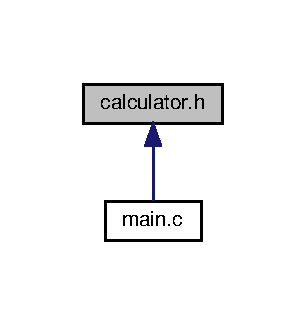
\includegraphics[width=147pt]{calculator_8h__dep__incl}
\end{center}
\end{figure}
\subsection*{Functions}
\begin{DoxyCompactItemize}
\item 
int \hyperlink{calculator_8h_a276d9db46d4c5b241b5b75e50646daf4}{calc} (int $\ast$)
\begin{DoxyCompactList}\small\item\em calculator function to evaluate postifx expression \end{DoxyCompactList}\end{DoxyCompactItemize}


\subsection{Detailed Description}
Header file for Calculator. 

\begin{DoxyDate}{Date}
2018/06/10 
\end{DoxyDate}
\begin{DoxyAuthor}{Author}
Youngeun Park 
\end{DoxyAuthor}


\subsection{Function Documentation}
\mbox{\Hypertarget{calculator_8h_a276d9db46d4c5b241b5b75e50646daf4}\label{calculator_8h_a276d9db46d4c5b241b5b75e50646daf4}} 
\index{calculator.\+h@{calculator.\+h}!calc@{calc}}
\index{calc@{calc}!calculator.\+h@{calculator.\+h}}
\subsubsection{\texorpdfstring{calc()}{calc()}}
{\footnotesize\ttfamily int calc (\begin{DoxyParamCaption}\item[{int $\ast$}]{result }\end{DoxyParamCaption})}



calculator function to evaluate postifx expression 

\begin{DoxyReturn}{Returns}
On success, 1~\newline
On failure, 0
\end{DoxyReturn}

\begin{DoxyParams}{Parameters}
{\em result} & (O\+UT) \+: integer pointer to return calculated result \\
\hline
\end{DoxyParams}

\hypertarget{convert_8c}{}\section{convert.\+c File Reference}
\label{convert_8c}\index{convert.\+c@{convert.\+c}}


\hyperlink{convert_8c}{convert.\+c}  


{\ttfamily \#include $<$stdio.\+h$>$}\newline
{\ttfamily \#include $<$stdlib.\+h$>$}\newline
{\ttfamily \#include $<$string.\+h$>$}\newline
{\ttfamily \#include $<$buffer.\+h$>$}\newline
{\ttfamily \#include $<$stack.\+h$>$}\newline
Include dependency graph for convert.\+c\+:\nopagebreak
\begin{figure}[H]
\begin{center}
\leavevmode
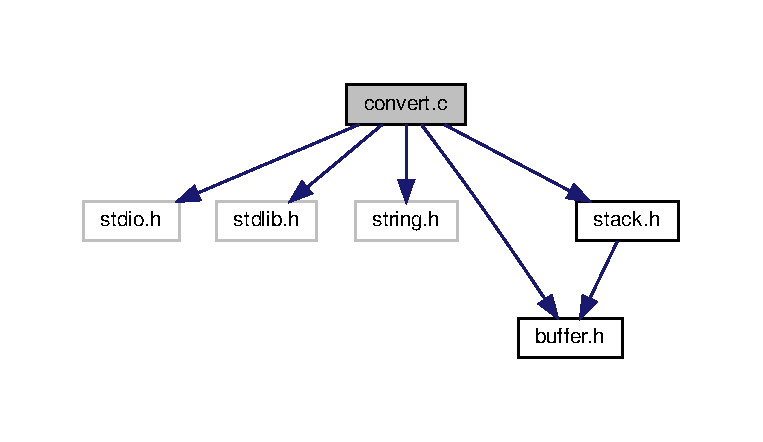
\includegraphics[width=350pt]{convert_8c__incl}
\end{center}
\end{figure}
\subsection*{Macros}
\begin{DoxyCompactItemize}
\item 
\mbox{\Hypertarget{convert_8c_a72032b867b0c9f8eab108a7210892990}\label{convert_8c_a72032b867b0c9f8eab108a7210892990}} 
\#define {\bfseries is\+Numeric}(c)~((c $>$= \textquotesingle{}0\textquotesingle{}) \&\& (c $<$= \textquotesingle{}9\textquotesingle{}))
\item 
\mbox{\Hypertarget{convert_8c_a44f7c035009c45eacb8d7c8680e4dddd}\label{convert_8c_a44f7c035009c45eacb8d7c8680e4dddd}} 
\#define {\bfseries to\+Numeric}(c)~(c -\/ \textquotesingle{}0\textquotesingle{})
\item 
\mbox{\Hypertarget{convert_8c_a5fd3acbdba0ff2963d05d6af8bcff181}\label{convert_8c_a5fd3acbdba0ff2963d05d6af8bcff181}} 
\#define {\bfseries is\+Terminator}(c)~((c == \textquotesingle{}\textbackslash{}n\textquotesingle{}) $\vert$$\vert$ (c == 0))
\item 
\mbox{\Hypertarget{convert_8c_a51b973b0dd5272bb97f9d9c9aff18c36}\label{convert_8c_a51b973b0dd5272bb97f9d9c9aff18c36}} 
\#define {\bfseries is\+White\+Char}(c)~((c == \textquotesingle{} \textquotesingle{}) $\vert$$\vert$ (c == \textquotesingle{}\textbackslash{}t\textquotesingle{}))
\end{DoxyCompactItemize}
\subsection*{Functions}
\begin{DoxyCompactItemize}
\item 
int \hyperlink{convert_8c_a9eee13860c4c03eac3f53c3a1f3aba80}{convert\+To\+Post\+Fix} (void)
\begin{DoxyCompactList}\small\item\em Convert infix expression into postpix one. \end{DoxyCompactList}\end{DoxyCompactItemize}


\subsection{Detailed Description}
\hyperlink{convert_8c}{convert.\+c} 

\begin{DoxyDate}{Date}
2018/06/10 
\end{DoxyDate}
\begin{DoxyAuthor}{Author}
Youngeun Park 
\end{DoxyAuthor}


\subsection{Function Documentation}
\mbox{\Hypertarget{convert_8c_a9eee13860c4c03eac3f53c3a1f3aba80}\label{convert_8c_a9eee13860c4c03eac3f53c3a1f3aba80}} 
\index{convert.\+c@{convert.\+c}!convert\+To\+Post\+Fix@{convert\+To\+Post\+Fix}}
\index{convert\+To\+Post\+Fix@{convert\+To\+Post\+Fix}!convert.\+c@{convert.\+c}}
\subsubsection{\texorpdfstring{convert\+To\+Post\+Fix()}{convertToPostFix()}}
{\footnotesize\ttfamily int convert\+To\+Post\+Fix (\begin{DoxyParamCaption}\item[{void}]{ }\end{DoxyParamCaption})}



Convert infix expression into postpix one. 

\+: the number of operators on success -\/1 on failure 
\hypertarget{convert_8h}{}\section{convert.\+h File Reference}
\label{convert_8h}\index{convert.\+h@{convert.\+h}}


Convert.\+h.  


This graph shows which files directly or indirectly include this file\+:\nopagebreak
\begin{figure}[H]
\begin{center}
\leavevmode
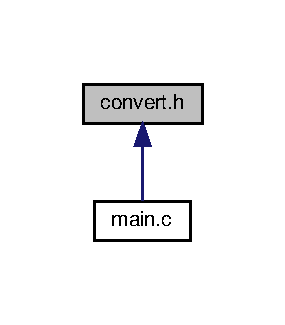
\includegraphics[width=137pt]{convert_8h__dep__incl}
\end{center}
\end{figure}
\subsection*{Functions}
\begin{DoxyCompactItemize}
\item 
int \hyperlink{convert_8h_a9eee13860c4c03eac3f53c3a1f3aba80}{convert\+To\+Post\+Fix} (void)
\end{DoxyCompactItemize}


\subsection{Detailed Description}
Convert.\+h. 

\begin{DoxyDate}{Date}
2018/06/10 
\end{DoxyDate}
\begin{DoxyAuthor}{Author}
Youngeun Park 
\end{DoxyAuthor}


\subsection{Function Documentation}
\mbox{\Hypertarget{convert_8h_a9eee13860c4c03eac3f53c3a1f3aba80}\label{convert_8h_a9eee13860c4c03eac3f53c3a1f3aba80}} 
\index{convert.\+h@{convert.\+h}!convert\+To\+Post\+Fix@{convert\+To\+Post\+Fix}}
\index{convert\+To\+Post\+Fix@{convert\+To\+Post\+Fix}!convert.\+h@{convert.\+h}}
\subsubsection{\texorpdfstring{convert\+To\+Post\+Fix()}{convertToPostFix()}}
{\footnotesize\ttfamily int convert\+To\+Post\+Fix (\begin{DoxyParamCaption}\item[{void}]{ }\end{DoxyParamCaption})}

Convert infix expression into postpix~\newline
( Reference\+: \href{https://www.tutorialspoint.com/data_structures_algorithms/expression_parsing.htm}{\tt https\+://www.\+tutorialspoint.\+com/data\+\_\+structures\+\_\+algorithms/expression\+\_\+parsing.\+htm} )

\begin{DoxyReturn}{Returns}
On success, the number of operators to be parsed~\newline
On failutre, -\/1 
\end{DoxyReturn}

\hypertarget{main_8c}{}\section{main.\+c File Reference}
\label{main_8c}\index{main.\+c@{main.\+c}}


Calculator program reads the string of numeric infix expression, converts it postfix expression, calculates the postfix expression and prints out the result.  


{\ttfamily \#include $<$stdio.\+h$>$}\newline
{\ttfamily \#include $<$stdlib.\+h$>$}\newline
{\ttfamily \#include $<$buffer.\+h$>$}\newline
{\ttfamily \#include $<$convert.\+h$>$}\newline
{\ttfamily \#include $<$calculator.\+h$>$}\newline
Include dependency graph for main.\+c\+:\nopagebreak
\begin{figure}[H]
\begin{center}
\leavevmode
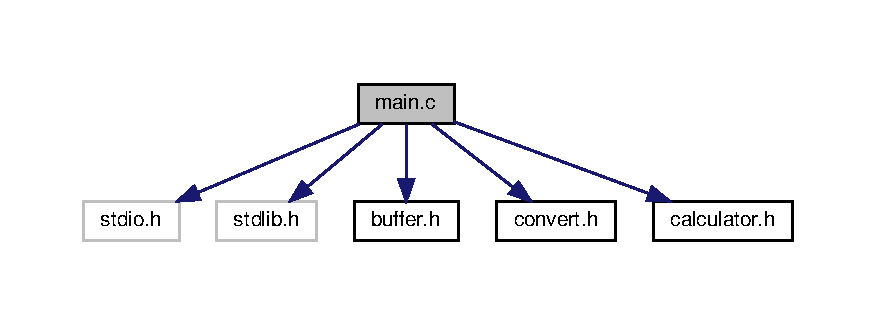
\includegraphics[width=350pt]{main_8c__incl}
\end{center}
\end{figure}
\subsection*{Functions}
\begin{DoxyCompactItemize}
\item 
int \hyperlink{main_8c_a840291bc02cba5474a4cb46a9b9566fe}{main} (void)
\end{DoxyCompactItemize}


\subsection{Detailed Description}
Calculator program reads the string of numeric infix expression, converts it postfix expression, calculates the postfix expression and prints out the result. 

\begin{DoxyDate}{Date}
2018/06/10 
\end{DoxyDate}
\begin{DoxyAuthor}{Author}
Youngeun Park 
\end{DoxyAuthor}


\subsection{Function Documentation}
\mbox{\Hypertarget{main_8c_a840291bc02cba5474a4cb46a9b9566fe}\label{main_8c_a840291bc02cba5474a4cb46a9b9566fe}} 
\index{main.\+c@{main.\+c}!main@{main}}
\index{main@{main}!main.\+c@{main.\+c}}
\subsubsection{\texorpdfstring{main()}{main()}}
{\footnotesize\ttfamily int main (\begin{DoxyParamCaption}\item[{void}]{ }\end{DoxyParamCaption})}

\begin{DoxyReturn}{Returns}

\end{DoxyReturn}

\hypertarget{stack_8c}{}\section{stack.\+c File Reference}
\label{stack_8c}\index{stack.\+c@{stack.\+c}}


\hyperlink{stack_8c}{stack.\+c}  


{\ttfamily \#include $<$string.\+h$>$}\newline
{\ttfamily \#include $<$stack.\+h$>$}\newline
Include dependency graph for stack.\+c\+:\nopagebreak
\begin{figure}[H]
\begin{center}
\leavevmode
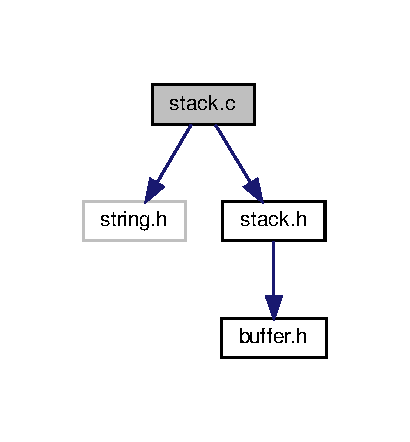
\includegraphics[width=197pt]{stack_8c__incl}
\end{center}
\end{figure}
\subsection*{Functions}
\begin{DoxyCompactItemize}
\item 
\mbox{\Hypertarget{stack_8c_adde2633a88991d4b1d7ed6b86a9ade61}\label{stack_8c_adde2633a88991d4b1d7ed6b86a9ade61}} 
void {\bfseries push} (\hyperlink{struct__postfixT}{\+\_\+postfixT} c)
\item 
\mbox{\Hypertarget{stack_8c_a642510ff51d97d8ac363fd8f17f540b7}\label{stack_8c_a642510ff51d97d8ac363fd8f17f540b7}} 
void {\bfseries pop} (\hyperlink{struct__postfixT}{\+\_\+postfixT} $\ast$p)
\item 
\mbox{\Hypertarget{stack_8c_af632f511735fd5559f717751a3b2cb27}\label{stack_8c_af632f511735fd5559f717751a3b2cb27}} 
\hyperlink{struct__postfixT}{\+\_\+postfixT} {\bfseries top} (void)
\item 
\mbox{\Hypertarget{stack_8c_a4667371cc1652ec25dfec478a952c717}\label{stack_8c_a4667371cc1652ec25dfec478a952c717}} 
int {\bfseries empty} (void)
\item 
\mbox{\Hypertarget{stack_8c_a524d97c94164a24e4d4a8e09622788a5}\label{stack_8c_a524d97c94164a24e4d4a8e09622788a5}} 
void {\bfseries init\+Stack} (void)
\end{DoxyCompactItemize}


\subsection{Detailed Description}
\hyperlink{stack_8c}{stack.\+c} 

\begin{DoxyDate}{Date}
2018/06/10 
\end{DoxyDate}
\begin{DoxyAuthor}{Author}
Youngeun Park 
\end{DoxyAuthor}

\hypertarget{stack_8cpp}{}\section{stack.\+cpp File Reference}
\label{stack_8cpp}\index{stack.\+cpp@{stack.\+cpp}}


C++ \hyperlink{classStack}{Stack} implementation for symbols.  


{\ttfamily \#include $<$iostream$>$}\newline
{\ttfamily \#include $<$string.\+h$>$}\newline
{\ttfamily \#include $<$stdlib.\+h$>$}\newline
{\ttfamily \#include $<$stack.\+hpp$>$}\newline
Include dependency graph for stack.\+cpp\+:
\nopagebreak
\begin{figure}[H]
\begin{center}
\leavevmode
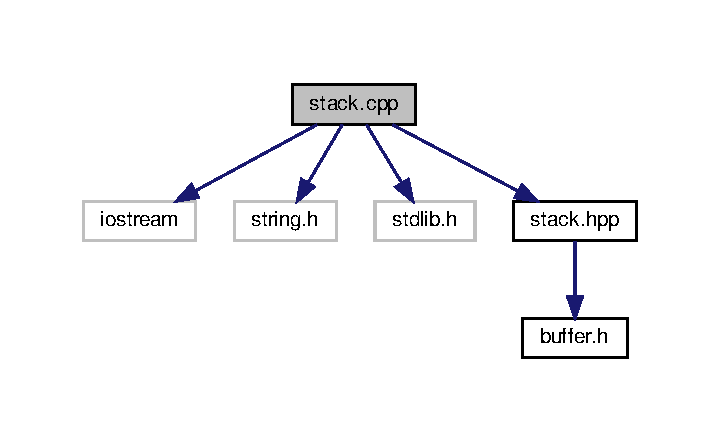
\includegraphics[width=346pt]{stack_8cpp__incl}
\end{center}
\end{figure}


\subsection{Detailed Description}
C++ \hyperlink{classStack}{Stack} implementation for symbols. 

\begin{DoxyDate}{Date}
2018/06/10 
\end{DoxyDate}
\begin{DoxyAuthor}{Author}
Youngeun Park 
\end{DoxyAuthor}

\hypertarget{stack_8h}{}\section{stack.\+h File Reference}
\label{stack_8h}\index{stack.\+h@{stack.\+h}}


header file for stack implementation  


{\ttfamily \#include $<$buffer.\+h$>$}\newline
Include dependency graph for stack.\+h\+:\nopagebreak
\begin{figure}[H]
\begin{center}
\leavevmode
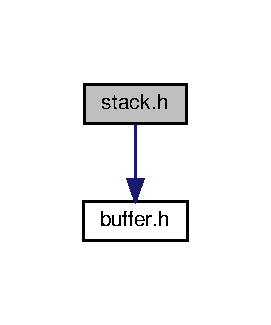
\includegraphics[width=130pt]{stack_8h__incl}
\end{center}
\end{figure}
This graph shows which files directly or indirectly include this file\+:\nopagebreak
\begin{figure}[H]
\begin{center}
\leavevmode
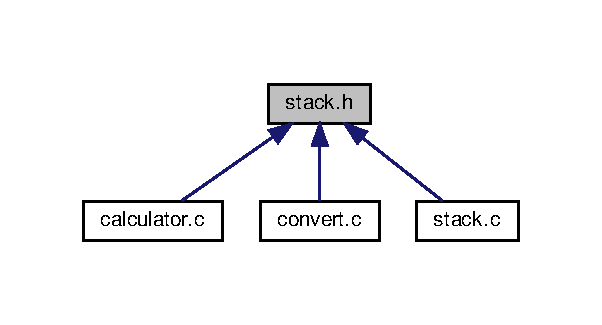
\includegraphics[width=289pt]{stack_8h__dep__incl}
\end{center}
\end{figure}
\subsection*{Functions}
\begin{DoxyCompactItemize}
\item 
void \hyperlink{stack_8h_a28fa2e71ac1a03e48f6393e614e9700d}{push} (\hyperlink{structsymbolT}{symbolT} c)
\begin{DoxyCompactList}\small\item\em Push symbol onto stack. \end{DoxyCompactList}\item 
void \hyperlink{stack_8h_ad2c9ad0bb34ef89958ab15329fb47222}{pop} (\hyperlink{structsymbolT}{symbolT} $\ast$p)
\begin{DoxyCompactList}\small\item\em Pop symbol from stack. \end{DoxyCompactList}\item 
\hyperlink{structsymbolT}{symbolT} \hyperlink{stack_8h_adc8484c9203490f40d71ecf61d47a8aa}{top} (void)
\begin{DoxyCompactList}\small\item\em Peek symbol on stack top. \end{DoxyCompactList}\item 
int \hyperlink{stack_8h_a4667371cc1652ec25dfec478a952c717}{empty} (void)
\begin{DoxyCompactList}\small\item\em Check if stack is empty. \end{DoxyCompactList}\item 
int \hyperlink{stack_8h_afe4b1c4ca08318016497caf30ad9e0f3}{full} (void)
\begin{DoxyCompactList}\small\item\em Check if stack is full. \end{DoxyCompactList}\item 
void \hyperlink{stack_8h_a524d97c94164a24e4d4a8e09622788a5}{init\+Stack} (void)
\begin{DoxyCompactList}\small\item\em Initialize stack. \end{DoxyCompactList}\end{DoxyCompactItemize}


\subsection{Detailed Description}
header file for stack implementation 

\begin{DoxyDate}{Date}
2018/06/10 
\end{DoxyDate}
\begin{DoxyAuthor}{Author}
Youngeun Park 
\end{DoxyAuthor}


\subsection{Function Documentation}
\mbox{\Hypertarget{stack_8h_a4667371cc1652ec25dfec478a952c717}\label{stack_8h_a4667371cc1652ec25dfec478a952c717}} 
\index{stack.\+h@{stack.\+h}!empty@{empty}}
\index{empty@{empty}!stack.\+h@{stack.\+h}}
\subsubsection{\texorpdfstring{empty()}{empty()}}
{\footnotesize\ttfamily int empty (\begin{DoxyParamCaption}\item[{void}]{ }\end{DoxyParamCaption})}



Check if stack is empty. 

\begin{DoxyReturn}{Returns}
1, if stack is empty~\newline
0, otherwise
\end{DoxyReturn}

\begin{DoxyParams}{Parameters}
{\em N\+O\+NE} & \\
\hline
\end{DoxyParams}
\mbox{\Hypertarget{stack_8h_afe4b1c4ca08318016497caf30ad9e0f3}\label{stack_8h_afe4b1c4ca08318016497caf30ad9e0f3}} 
\index{stack.\+h@{stack.\+h}!full@{full}}
\index{full@{full}!stack.\+h@{stack.\+h}}
\subsubsection{\texorpdfstring{full()}{full()}}
{\footnotesize\ttfamily int full (\begin{DoxyParamCaption}\item[{void}]{ }\end{DoxyParamCaption})}



Check if stack is full. 

\begin{DoxyReturn}{Returns}
1, if stack is empty~\newline
0, otherwise
\end{DoxyReturn}

\begin{DoxyParams}{Parameters}
{\em N\+O\+NE} & \\
\hline
\end{DoxyParams}
\mbox{\Hypertarget{stack_8h_a524d97c94164a24e4d4a8e09622788a5}\label{stack_8h_a524d97c94164a24e4d4a8e09622788a5}} 
\index{stack.\+h@{stack.\+h}!init\+Stack@{init\+Stack}}
\index{init\+Stack@{init\+Stack}!stack.\+h@{stack.\+h}}
\subsubsection{\texorpdfstring{init\+Stack()}{initStack()}}
{\footnotesize\ttfamily void init\+Stack (\begin{DoxyParamCaption}\item[{void}]{ }\end{DoxyParamCaption})}



Initialize stack. 

\begin{DoxyReturn}{Returns}
N\+O\+NE
\end{DoxyReturn}

\begin{DoxyParams}{Parameters}
{\em N\+O\+NE} & \\
\hline
\end{DoxyParams}
\mbox{\Hypertarget{stack_8h_ad2c9ad0bb34ef89958ab15329fb47222}\label{stack_8h_ad2c9ad0bb34ef89958ab15329fb47222}} 
\index{stack.\+h@{stack.\+h}!pop@{pop}}
\index{pop@{pop}!stack.\+h@{stack.\+h}}
\subsubsection{\texorpdfstring{pop()}{pop()}}
{\footnotesize\ttfamily void pop (\begin{DoxyParamCaption}\item[{\hyperlink{structsymbolT}{symbolT} $\ast$}]{p }\end{DoxyParamCaption})}



Pop symbol from stack. 

\begin{DoxyReturn}{Returns}
N\+O\+NE
\end{DoxyReturn}

\begin{DoxyParams}{Parameters}
{\em p} & \+: pointer of symbol to return the symbol on stack top \\
\hline
\end{DoxyParams}
\mbox{\Hypertarget{stack_8h_a28fa2e71ac1a03e48f6393e614e9700d}\label{stack_8h_a28fa2e71ac1a03e48f6393e614e9700d}} 
\index{stack.\+h@{stack.\+h}!push@{push}}
\index{push@{push}!stack.\+h@{stack.\+h}}
\subsubsection{\texorpdfstring{push()}{push()}}
{\footnotesize\ttfamily void push (\begin{DoxyParamCaption}\item[{\hyperlink{structsymbolT}{symbolT}}]{c }\end{DoxyParamCaption})}



Push symbol onto stack. 

\begin{DoxyReturn}{Returns}
N\+O\+NE
\end{DoxyReturn}

\begin{DoxyParams}{Parameters}
{\em c} & \+: symbol to push onto stack \\
\hline
\end{DoxyParams}
\mbox{\Hypertarget{stack_8h_adc8484c9203490f40d71ecf61d47a8aa}\label{stack_8h_adc8484c9203490f40d71ecf61d47a8aa}} 
\index{stack.\+h@{stack.\+h}!top@{top}}
\index{top@{top}!stack.\+h@{stack.\+h}}
\subsubsection{\texorpdfstring{top()}{top()}}
{\footnotesize\ttfamily \hyperlink{structsymbolT}{symbolT} top (\begin{DoxyParamCaption}\item[{void}]{ }\end{DoxyParamCaption})}



Peek symbol on stack top. 

\begin{DoxyReturn}{Returns}
symbol on stack top
\end{DoxyReturn}

\begin{DoxyParams}{Parameters}
{\em N\+O\+NE} & \\
\hline
\end{DoxyParams}

\hypertarget{stack_8hpp}{}\section{stack.\+hpp File Reference}
\label{stack_8hpp}\index{stack.\+hpp@{stack.\+hpp}}


C++ header file for stack implementation.  


{\ttfamily \#include $<$buffer.\+h$>$}\newline
Include dependency graph for stack.\+hpp\+:
\nopagebreak
\begin{figure}[H]
\begin{center}
\leavevmode
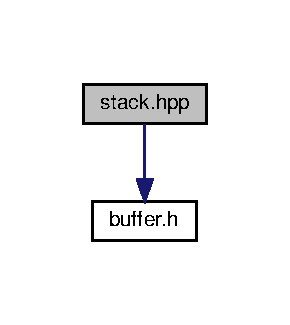
\includegraphics[width=139pt]{stack_8hpp__incl}
\end{center}
\end{figure}
This graph shows which files directly or indirectly include this file\+:
\nopagebreak
\begin{figure}[H]
\begin{center}
\leavevmode
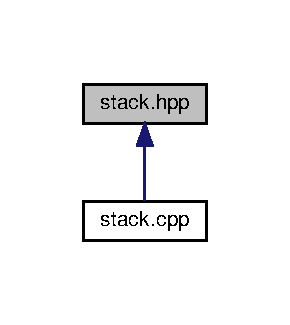
\includegraphics[width=139pt]{stack_8hpp__dep__incl}
\end{center}
\end{figure}
\subsection*{Classes}
\begin{DoxyCompactItemize}
\item 
class \hyperlink{classStack}{Stack}
\end{DoxyCompactItemize}
\subsection*{Macros}
\begin{DoxyCompactItemize}
\item 
\mbox{\Hypertarget{stack_8hpp_accbb358028675c83675d8b34c386268d}\label{stack_8hpp_accbb358028675c83675d8b34c386268d}} 
\#define {\bfseries M\+A\+X\+\_\+\+S\+T\+A\+C\+K\+\_\+\+S\+I\+ZE}~M\+A\+X\+\_\+\+S\+T\+R\+I\+NG
\end{DoxyCompactItemize}


\subsection{Detailed Description}
C++ header file for stack implementation. 

\begin{DoxyDate}{Date}
2018/06/10 
\end{DoxyDate}
\begin{DoxyAuthor}{Author}
Youngeun Park 
\end{DoxyAuthor}

\hypertarget{utility_8h}{}\section{utility.\+h File Reference}
\label{utility_8h}\index{utility.\+h@{utility.\+h}}


Utility macros.  


This graph shows which files directly or indirectly include this file\+:\nopagebreak
\begin{figure}[H]
\begin{center}
\leavevmode
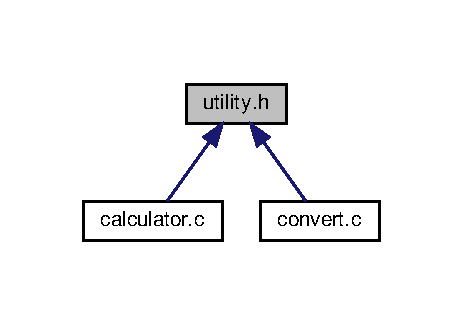
\includegraphics[width=222pt]{utility_8h__dep__incl}
\end{center}
\end{figure}
\subsection*{Macros}
\begin{DoxyCompactItemize}
\item 
\mbox{\Hypertarget{utility_8h_af01b43bbb0e04b9b0e9fd509f941deb8}\label{utility_8h_af01b43bbb0e04b9b0e9fd509f941deb8}} 
\#define \hyperlink{utility_8h_af01b43bbb0e04b9b0e9fd509f941deb8}{is\+Num}(c)~((c $>$= \textquotesingle{}0\textquotesingle{}) \&\& (c $<$= \textquotesingle{}9\textquotesingle{}))
\begin{DoxyCompactList}\small\item\em Check if given c is numeric number. \end{DoxyCompactList}\item 
\mbox{\Hypertarget{utility_8h_a5fd3acbdba0ff2963d05d6af8bcff181}\label{utility_8h_a5fd3acbdba0ff2963d05d6af8bcff181}} 
\#define \hyperlink{utility_8h_a5fd3acbdba0ff2963d05d6af8bcff181}{is\+Terminator}(c)~((c == \textquotesingle{}\textbackslash{}n\textquotesingle{}) $\vert$$\vert$ (c == 0))
\begin{DoxyCompactList}\small\item\em Check if given c is newline or N\+U\+LL. \end{DoxyCompactList}\item 
\mbox{\Hypertarget{utility_8h_ac975112ba9f532db68e2b1b3aa2efa89}\label{utility_8h_ac975112ba9f532db68e2b1b3aa2efa89}} 
\#define \hyperlink{utility_8h_ac975112ba9f532db68e2b1b3aa2efa89}{is\+Whitespace}(c)~((c == \textquotesingle{} \textquotesingle{}) $\vert$$\vert$ (c == \textquotesingle{}\textbackslash{}t\textquotesingle{}))
\begin{DoxyCompactList}\small\item\em Check if given c is white character. \end{DoxyCompactList}\item 
\mbox{\Hypertarget{utility_8h_a44f7c035009c45eacb8d7c8680e4dddd}\label{utility_8h_a44f7c035009c45eacb8d7c8680e4dddd}} 
\#define \hyperlink{utility_8h_a44f7c035009c45eacb8d7c8680e4dddd}{to\+Numeric}(c)~(c -\/ \textquotesingle{}0\textquotesingle{})
\begin{DoxyCompactList}\small\item\em Translate character c into integer value. \end{DoxyCompactList}\end{DoxyCompactItemize}


\subsection{Detailed Description}
Utility macros. 

\begin{DoxyDate}{Date}
2018/06/10 
\end{DoxyDate}
\begin{DoxyAuthor}{Author}
Youngeun Park 
\end{DoxyAuthor}

%--- End generated contents ---

% Index
\backmatter
\newpage
\phantomsection
\clearemptydoublepage
\addcontentsline{toc}{chapter}{Index}
\printindex

\end{document}
